\chapter{Typechecking}\label{ch:typechecking}
In the following chapter the purpose of the type checker will be elaborated. 
The definition and function of a type system will be defined and explained in relation to PHAL. 
Furthermore, the differences between static and dynamic type checking will be analysed. 
Finally, the type conversions and operator overloading will be analysed and related to PHAL in general terms.

\section{Purpose of the type checker}
A compiler must check whether the source program follows both the syntactic and semantic conventions of the given language. 
This type of checking is called static type checking, and ensures that certain kinds of programming errors will be detected and reported. 
As indicated by Figure~\ref{fig:TypeChecker}, the type check takes place between the parsing and the intermediate code generation.
\begin{figure}[H]
\centering
  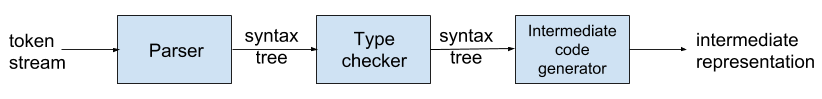
\includegraphics[width=0.8\textwidth]{figures/CompilerPhases/TypeChecker.png}
  \caption{This figure shows the position of the type checker in relation to the different compiler parses.}
  \label{fig:TypeChecker}
\end{figure}
The checks include, but are not limited to:
\begin{itemize}
    \item \textit{Type checks} - to see if an operation is applied to an incompatible operand.
    \item \textit{Flow-of-control checks} - statements that cause flow of control to leave a construct must have some place to transfer the flow of control.
    \item \textit{Uniqueness checks} - whether an object has been defined exactly once \cite{Dragon}.
\end{itemize}
If a given source program can pass the test of the type checker, it is said to be syntactically correct.

\section{Type systems}
When designing a type checker, multiple aspects of the language have to be considered, such as the syntactic constructs, the notation of types and rules for assigning types to language constructs. 

\subsection*{Type expressions}
The types of a language are denoted by type expressions. 
A type expression is either a basic type or is formed by applying an operator called a type constructor to other type expressions. 
The sets of basic types and constructors depend on the language that is subject to the check. 

\subsection*{Static and dynamic checking of types}
Type checking done at compile-time is called static type checking, whereas type checking done when the target program runs is called dynamic type checking.
If a language does not need dynamic type checking it is said to be \textit{sound}, because it allows us to statically determine that type errors can not occur on run time. 
\\\\
A language that is checked at compile time and can guarantee that the programs it accepts can be executed without any type errors is called a \textit{strongly typed} language \cite{Dragon}.

\subsection*{Error recovery}
Since the type checker has the potential to detect errors in the source program it needs the ability to take reasonable action when an error is discovered. At the very least the compiler should report the type and location of the error. However, it would be desirable for the type checker to be able to recover from an error and be able to check the rest of the program in order to detect any other potential errors before returning anything to the user.

\section{Type conversions}
During the type check it may be necessary to check conversions between types in most programming languages. 
Consider the expression $x+i$, where $x$ is of type \textit{integer} and $i$ is of type \textit{float}. In most languages it would be possible to convert $x$ to type \textit{float} since it would not result in missing precision.
\\\\
In PHAL this is mostly irrelevant since the abstraction of numbers has resulted in a single type to contain any kind of numbers. 
It would therefore not make sense to conduct type conversion in PHAL since \textit{integers} and \textit{floats} are the only similar data types.

\section{Overloading operators}
An overloaded symbol is one that takes on different meanings depending on the context in which it appears. 
For example, the $+$ is overloaded depending on context. In a mathematical context it would be used to imply addition of two numbers, however it can also be used on strings to perform a concatenation of them. In the same way, the dot operator is overloaded to either imply that a number is a \textit{float} or to access a \textit{sub-id} for an advanced type.
\\\\
The overloading of the $+$ operator in PHAL is described in Subsection~\ref{sem:aexp} and the other rules can be found in Appendix~\ref{app:semantics}.